\myappendix{Program Execution Screenshots}
%\addcontentsline{toc}{section}{Appendix D: Program Execution Screenshots}
\label{sec:appendix_D}

\begin{figure}[h!]
\centering
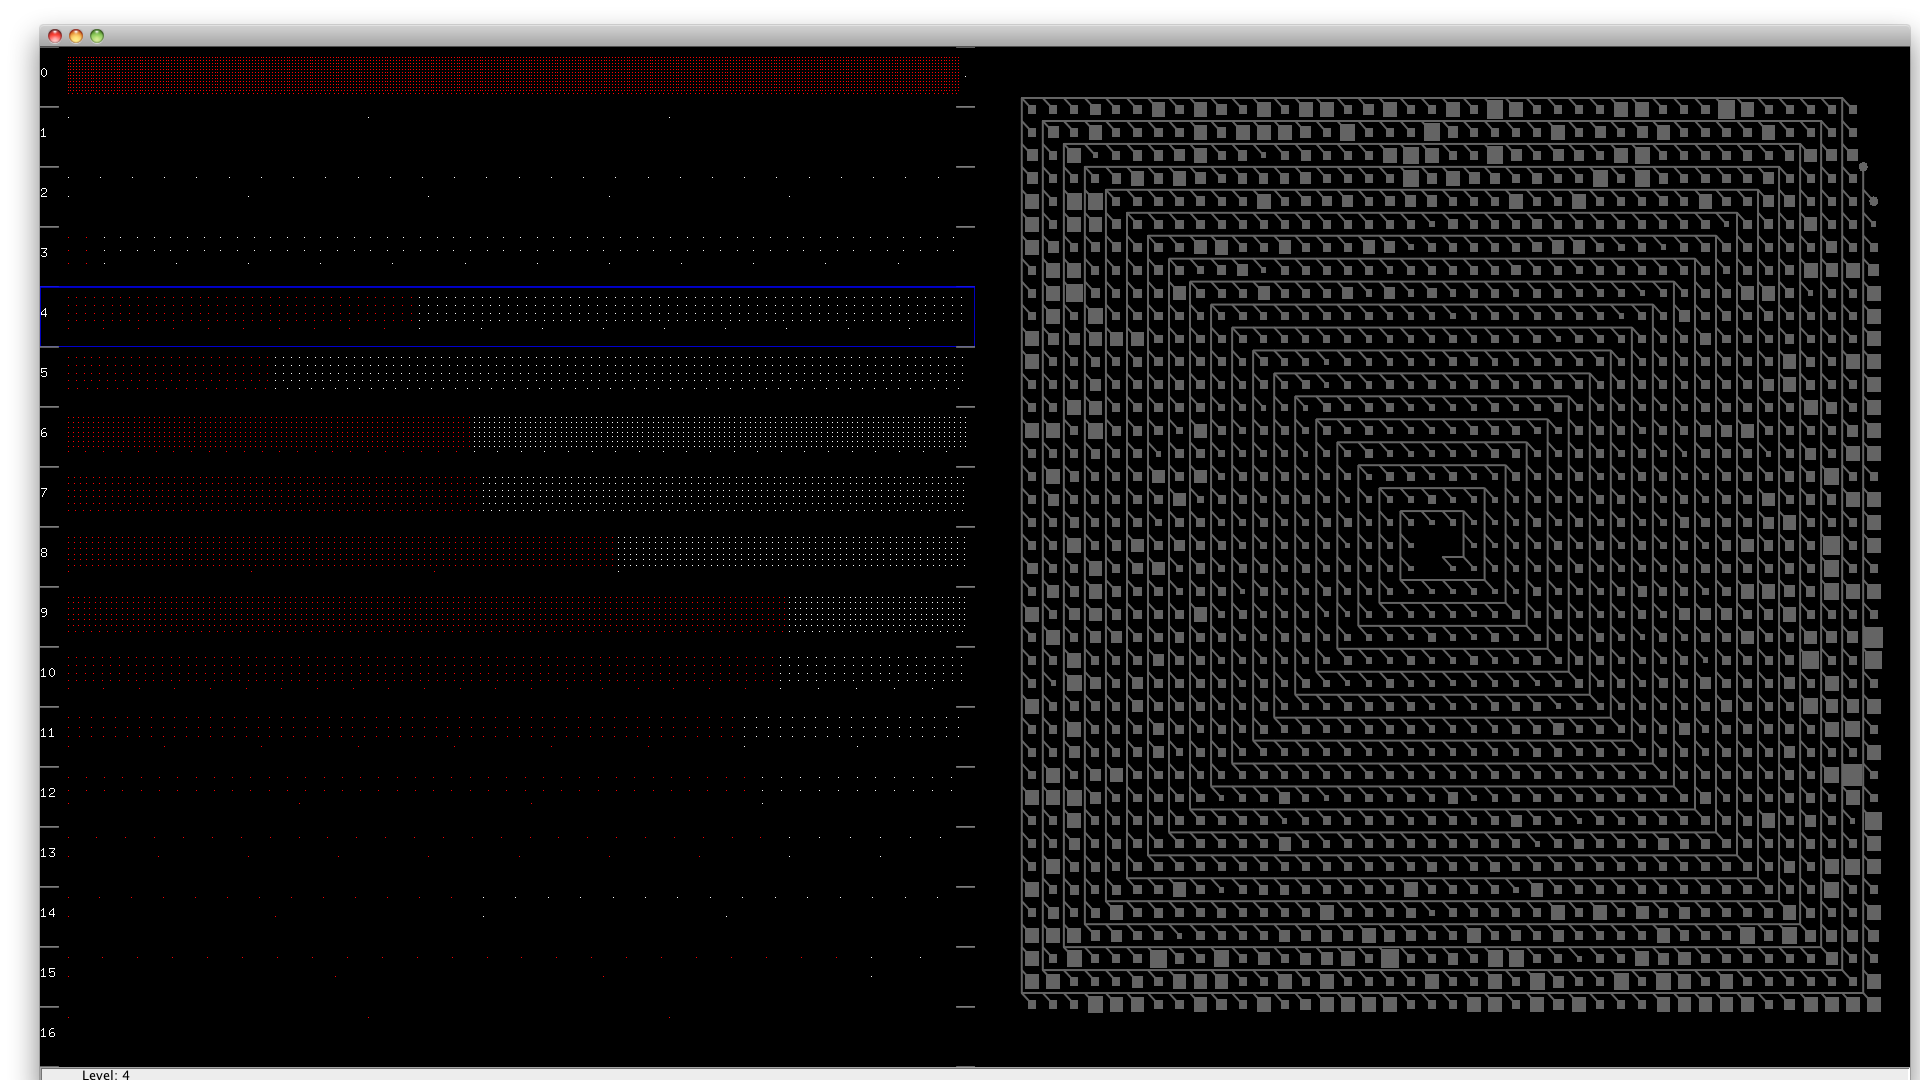
\includegraphics[scale=0.33, angle=90]{pictures/screenshot_1.png}
\caption{Visualization of the Gene Ontology graph by levels and Cluster analysis result graph. Blue rectangle -- highlighted level 4}
\end{figure}

\newpage
\begin{figure}[h!]
\centering
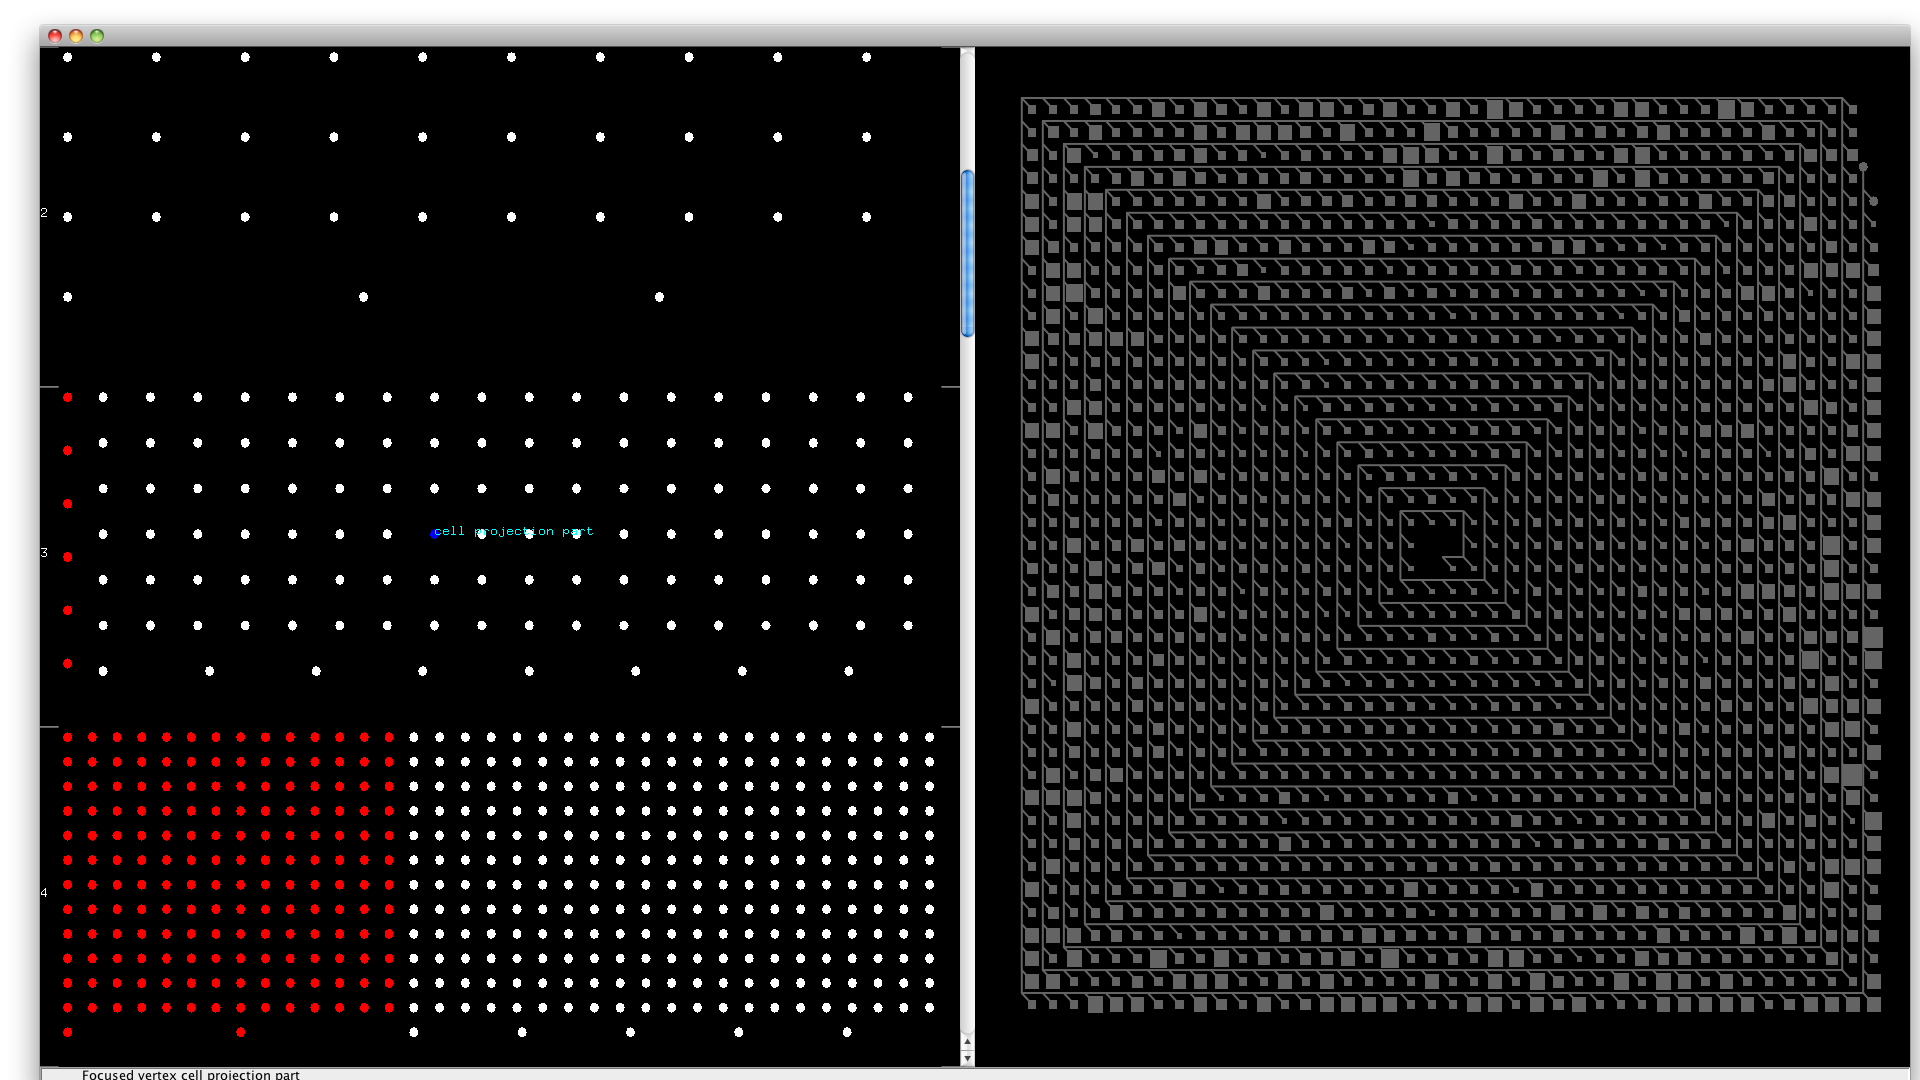
\includegraphics[scale=0.33, angle=90]{pictures/screenshot_2.png}
\caption{Zoomed visualizatoin of the Gene Ontology levels (2, 3 and 4) and focused vertex ``cell projection part"}
\end{figure}

\newpage
\begin{figure}[h!]
\centering
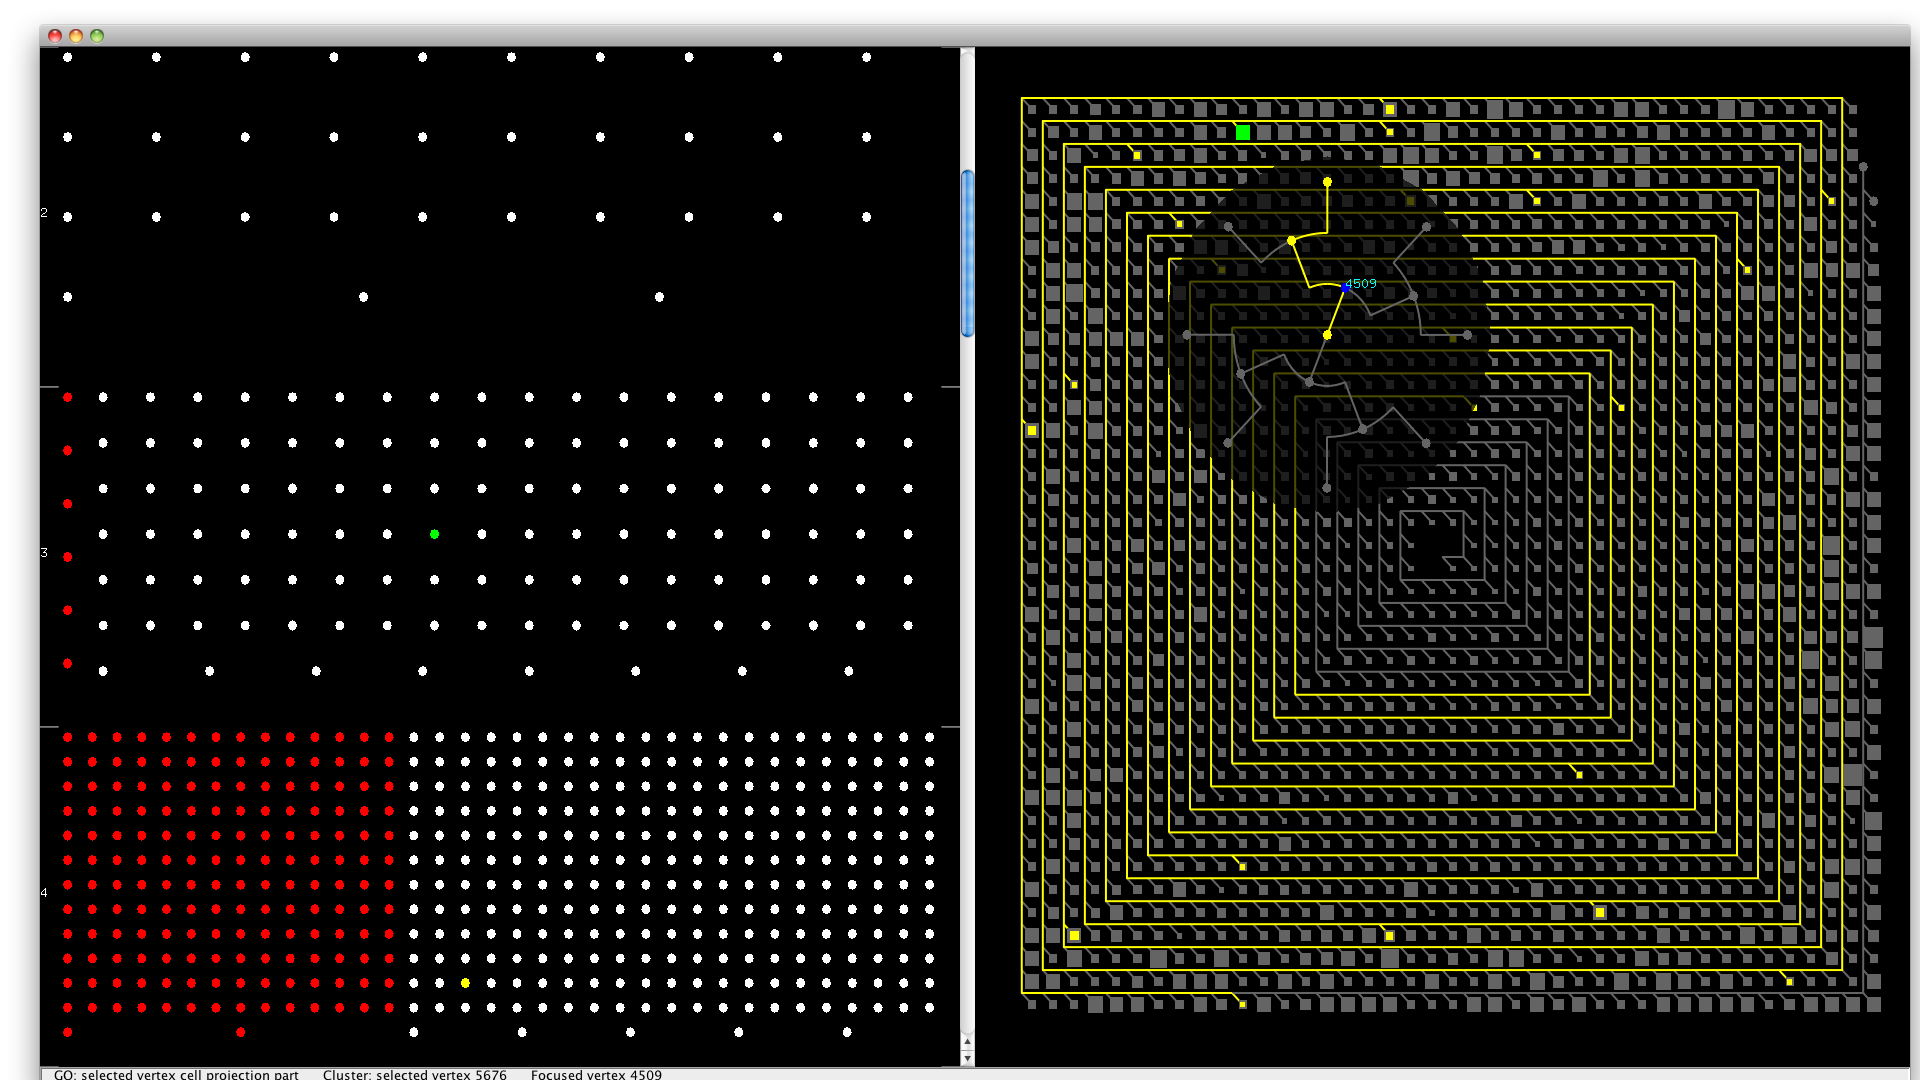
\includegraphics[scale=0.33, angle=90]{pictures/screenshot_3.png}
\caption{Highlighted sub-graph visualization for GO gene ``cell projection part" and Radial lens view of the Cluster grouped vertex ``5676" (green rectangle)}
\end{figure}

\newpage
\begin{figure}[h!]
\centering
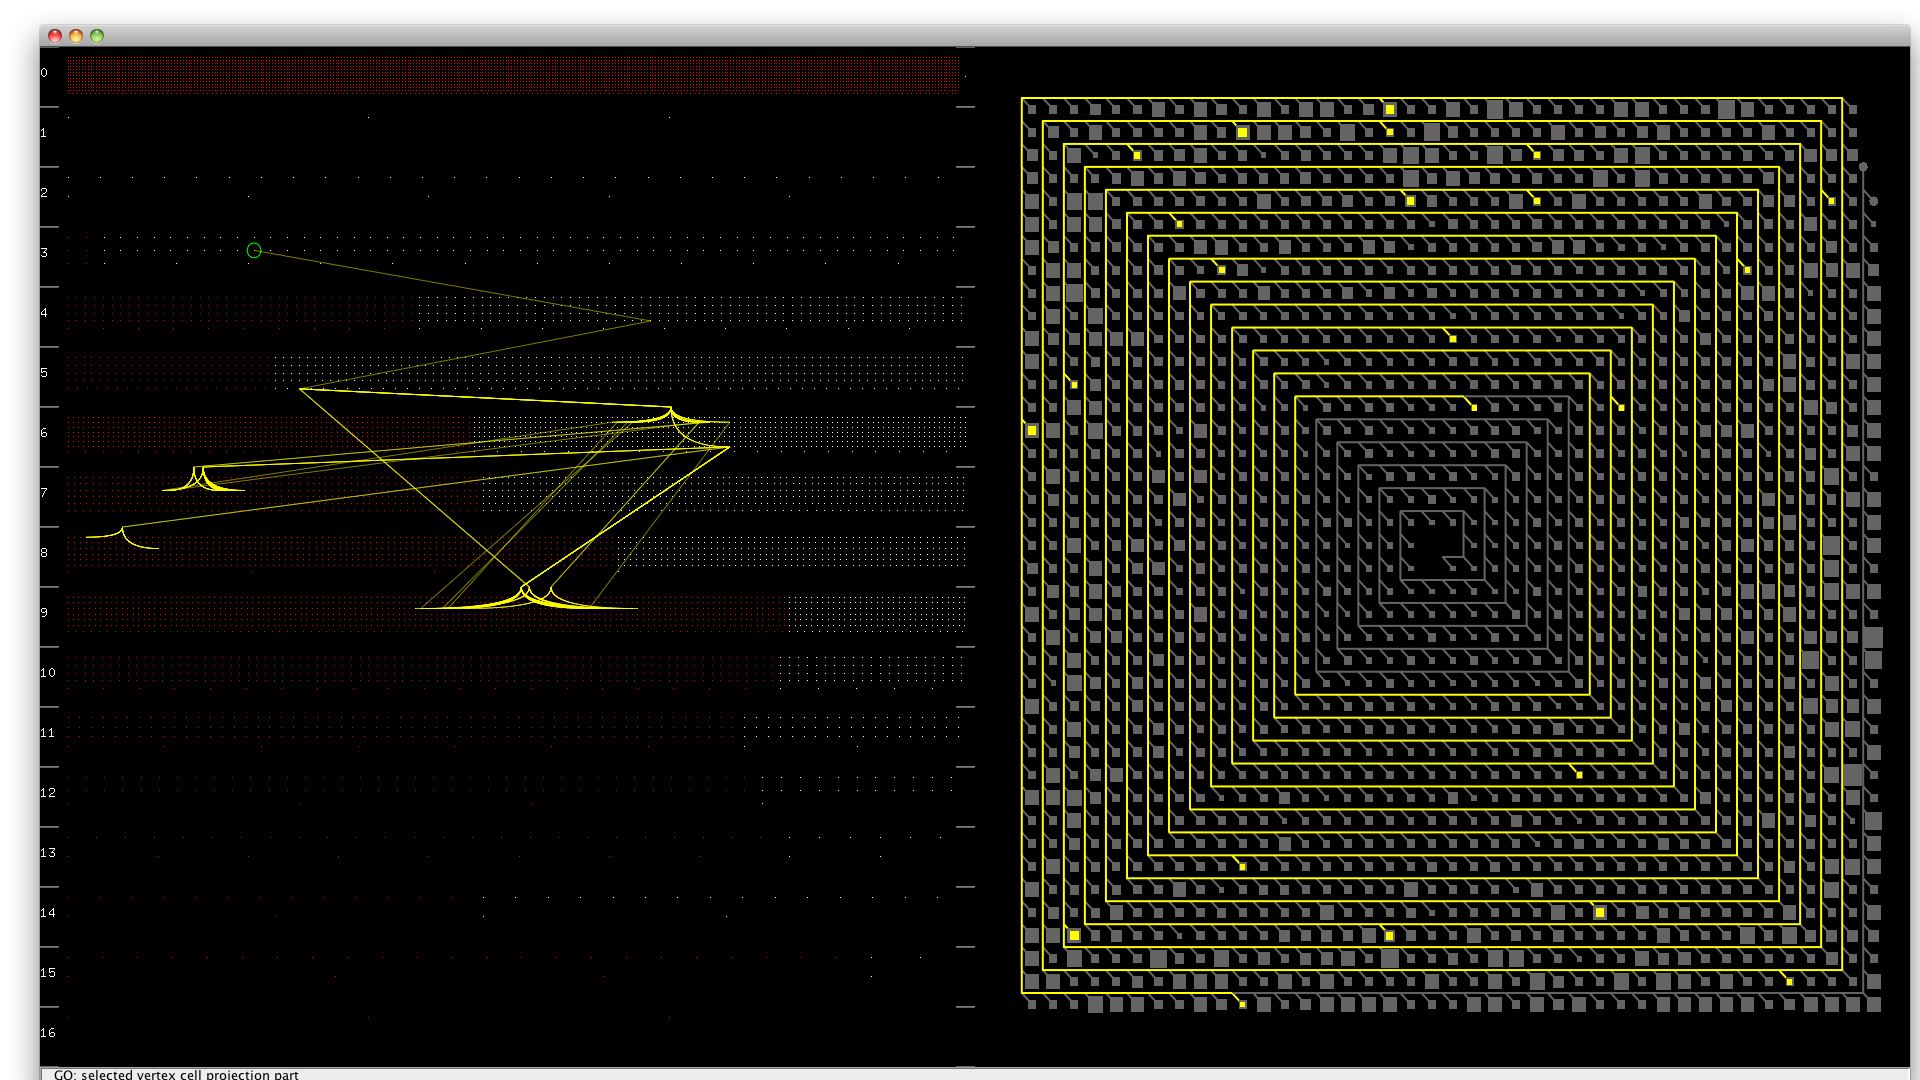
\includegraphics[scale=0.33, angle=90]{pictures/screenshot_4.png}
\caption{Highlighted sub-graph visualization for selected vertex ``cell projection part" (green circle)}
\end{figure}

\newpage
\begin{figure}[h!]
\centering
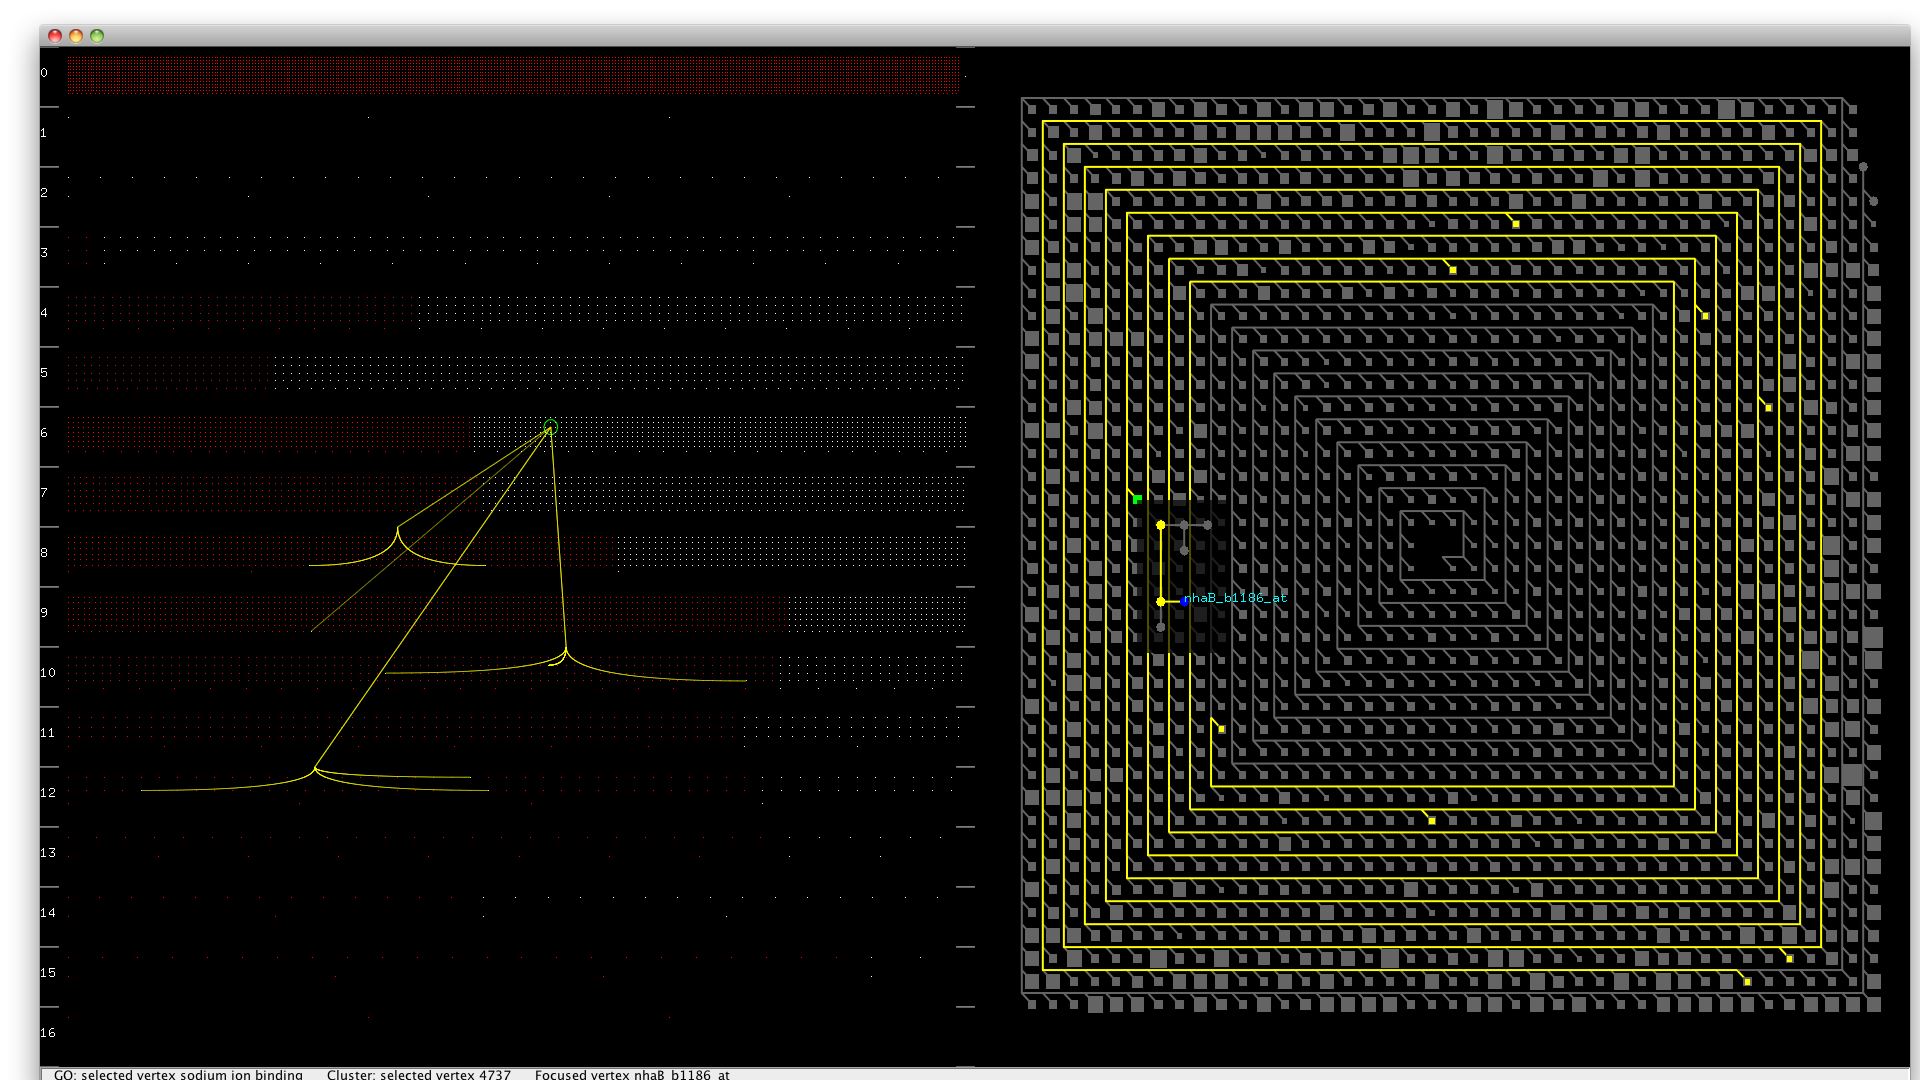
\includegraphics[scale=0.33, angle=90]{pictures/screenshot_5.png}
\caption{Highlighted sub-graph visualization for GO vertex ``sodium ion binding" and Rect lens view of the Cluster grouped vertex ``4737".}
\end{figure}

\newpage
\begin{figure}[h!]
\centering
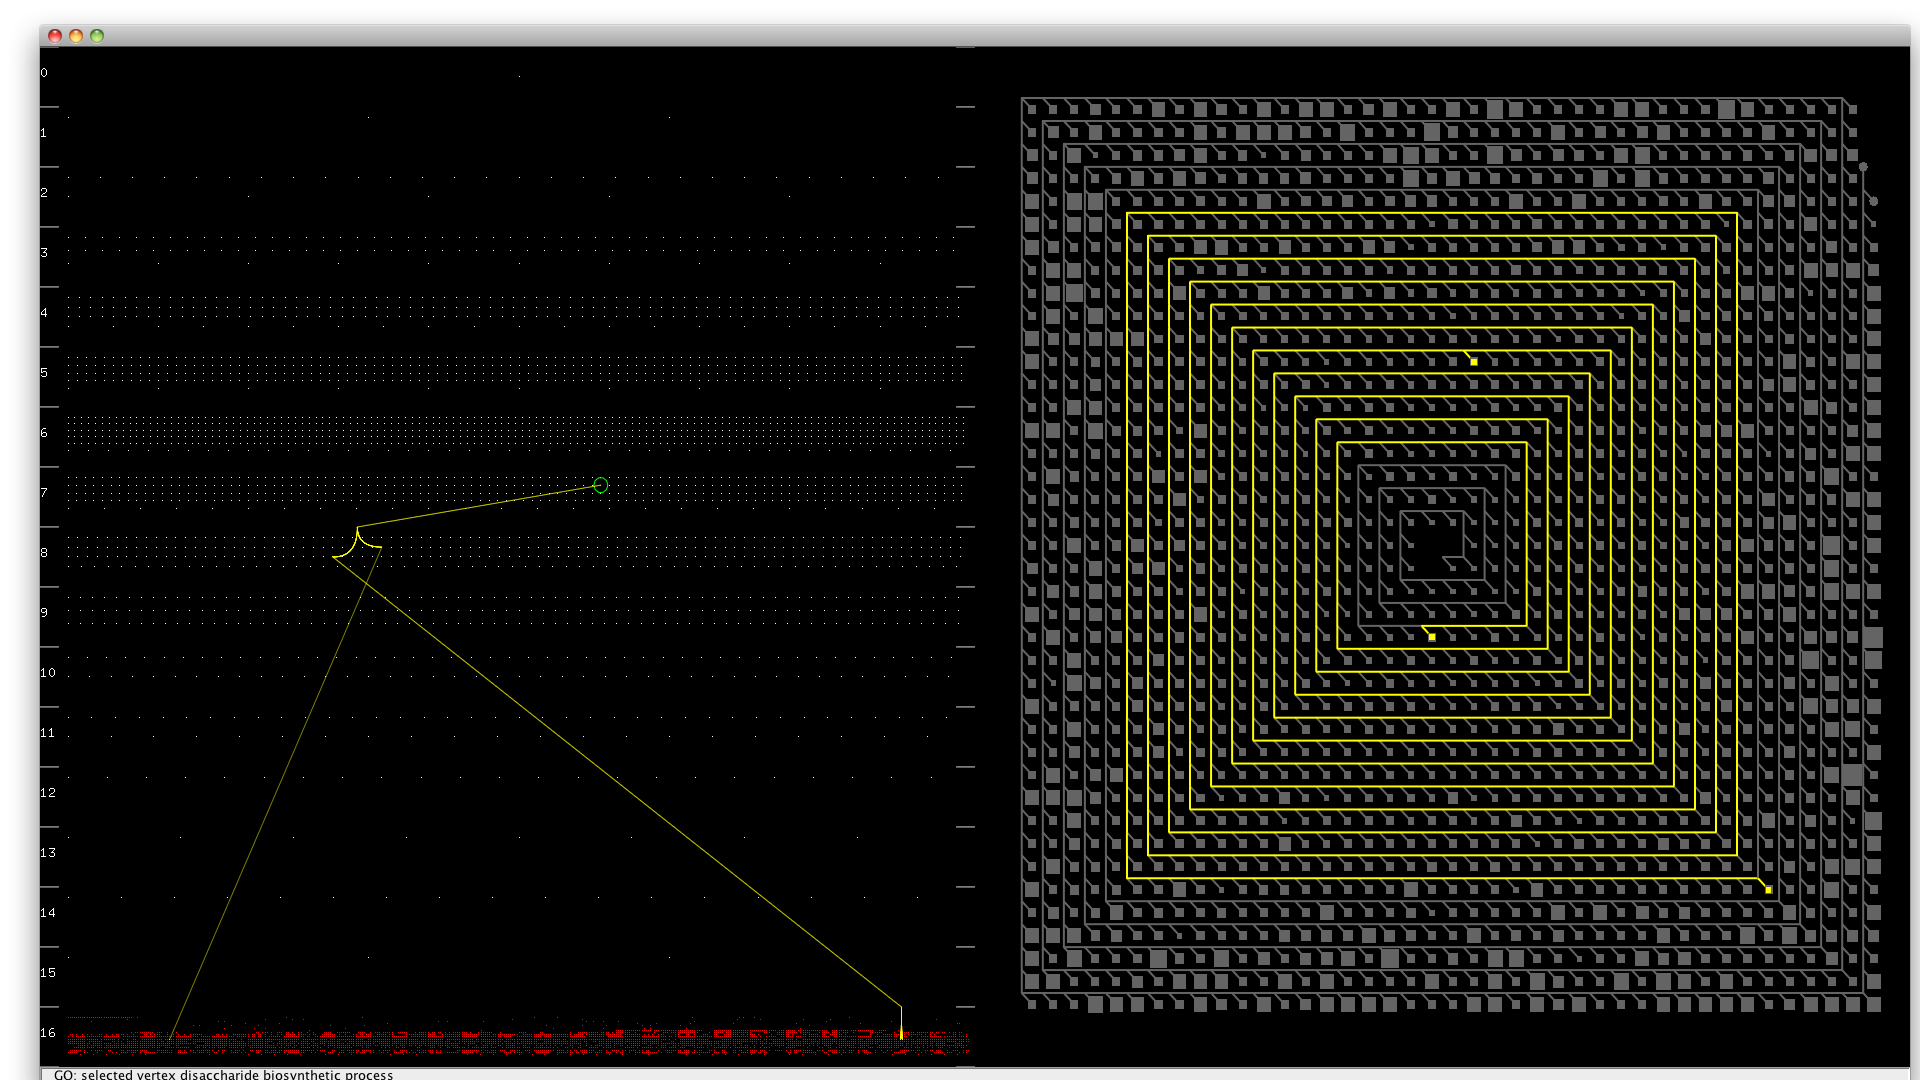
\includegraphics[scale=0.33, angle=90]{pictures/screenshot_6.png}
\caption{Visualization of the Gene Ontology graph using ``Leaf buttom layout" without option ``Show unconnected components" and highlighted sub-graph for the GO vertex ``disaccharide biosynthetic process"}
\end{figure}